\documentclass[tikz, border=10pt]{standalone}
\usetikzlibrary{backgrounds, chains, positioning, shadows,patterns}
\usepackage{standalone}

 \renewcommand{\familydefault}{\sfdefault}
%\fontfamily{helvetica}
  %\selectfont
  
\usepackage{pgfplots}
\usepgfplotslibrary{groupplots,fillbetween}
\usepackage{animate}
\usepackage{xcolor}

\usepackage{pgf}
\usepackage{tikz}

\usetikzlibrary{fit}
\usetikzlibrary{positioning}
\usetikzlibrary{arrows}
\usetikzlibrary{automata}
\usetikzlibrary{backgrounds}
\usetikzlibrary{shapes.misc}
\usetikzlibrary{decorations.pathreplacing,calligraphy}


\definecolor{orange}{HTML}{d95f02}
\definecolor{purple}{HTML}{7570b3}

\begin{document}
    \begin{tikzpicture}[
            node distance = 2cm, % distance between nodes
   start chain = going below,
               > = stealth, % arrow head style
            shorten > = 1pt, % don't touch arrow head to node
            auto,
          %  node distance = 2.5cm, % distance between nodes
            semithick, % line style
    box/.style = {rectangle, rounded corners, draw=gray, very thick,
                  minimum height=8mm, minimum width = 4 cm, align=flush center,
                  top color=#1!30, bottom color=#1!30},
   boxpattern/.style = {rectangle, rounded corners, draw=gray, very thick,
                  minimum height=8mm, minimum width = 4 cm, align=flush center,
                  pattern=north west lines, pattern color=#1},
    cir/.style = {circle, draw=black, very thick,
                  minimum size=16mm, inner sep=2pt, outer sep=0pt,
                  top color=white, bottom color=white},
   state/.style={ circle, draw = #1 ,
           very thick,
            fill = white,
            minimum size = 4mm},
            brace/.style={thick,decorate,
        decoration={calligraphic brace, amplitude=7pt,raise=0.5ex,mirror}}]
                        


% Data collection
\node (n1) [ box=white] {Seedlings};
\node (n2) [right =.25cm of n1, box=white] {Fruiting plants};
\node (n3) [right =.25cm of n2, box=white] {Fruits per plant};
\node (n4) [right =.25cm of n3, box=white]  {Seeds per fruit};

% Data structure
\node (d3) [box=white] at (.75,2)  {Plants in 30 permanent 0.5m$^2$ plots};
          \path[dotted] (n1) edge node {} (d3);
          \path[dotted] (n2) edge node {} (d3);
          \path[dotted] (n3) edge node {} (d3);
          
\node (d4) [ box=white] at (10.75,2)  {Plants in additional, haphazardly sampled 0.5m$^2$ plots};
          \path[dotted] (d4) edge node {} (n3);
          \path[dotted] (d4) edge node {} (n4);0

% Timeline
% \node[box=white,inner sep=.25pt,draw=black,minimum width = 2.25cm] (gantt) at (10.5,-1.5)
 %   {\includestandalone[scale=.45]{gantt}};          
          
% Observations
\node [below = .4 cm of n1,  cir=gray] (d1)    {$n^\mathrm{seedling}_{ijk}$};
\node [below = .4 cm of n2, cir=gray] (d2)   {$y^\mathrm{fruiting}_{ijk}$};

% connect observations to data
          \path[dotted] (n1) edge node {} (d1);
          \path[dotted] (n2) edge node {} (d2);

% SURVIVAL MODEL
       
          \path[dashed,->] (d1) edge node {} (d2);
                  
         % hyperparameters
         \node[state=none] (AB) [below of = d1] {$\alpha_{\mathrm{S},ijk}$};
                
         \path[->] (AB) edge node {} (d2);
         
          % hyperparameters
        
         \node[state=orange] (MS) [below of = AB] {$\mu_{\mathrm{S},jk}$};
         \node[state=orange] (A) [below left of = AB] {$\sigma_{\mathrm{S},jk}$};
         
         \path[->] (A) edge node {} (AB);       
         \path[->] (MS) edge node {} (AB);       
         
         \node[state=purple] (H) [below of = MS] {$\mu^\mathrm{pop}_{\mathrm{S},j},\sigma^\mathrm{pop}_{\mathrm{S},j}$};
         \path[->] (H) edge node {} (MS);       
         
\node[inner sep=0.25pt] (sigma) at (5.5,-6)
    {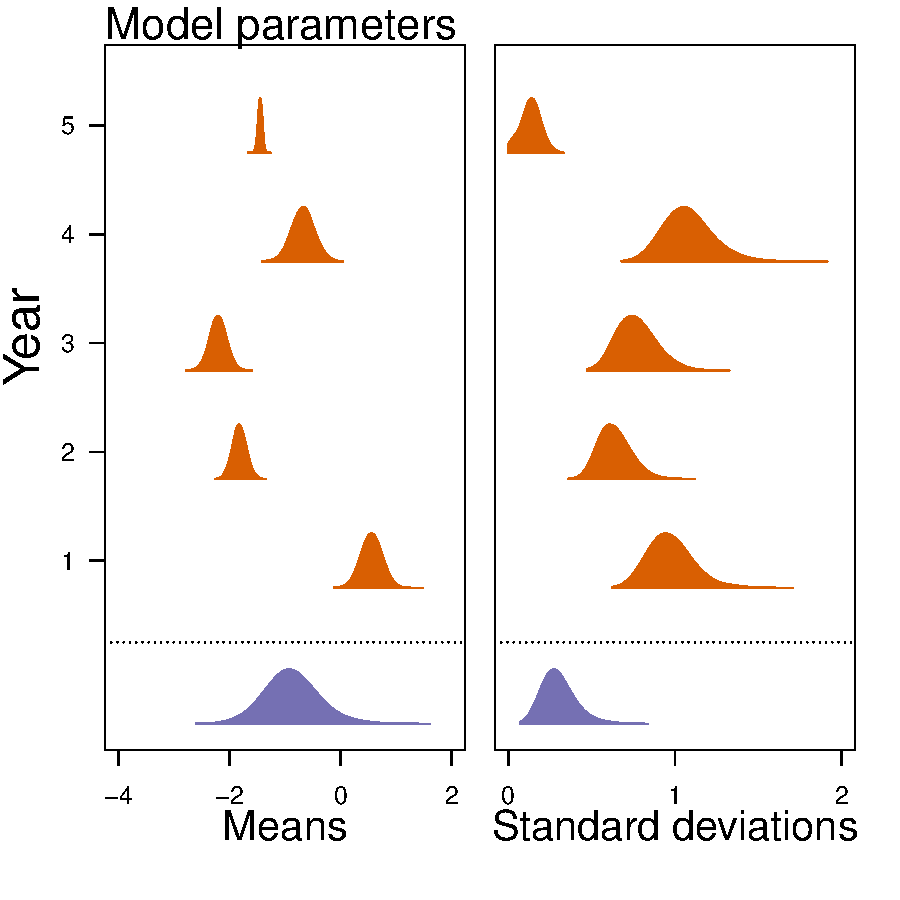
\includegraphics[trim={0 0 0 0},clip,scale=.4]{parameter}};
\node[inner sep=0.25pt] (sigma2) at (11.8,-6)
    {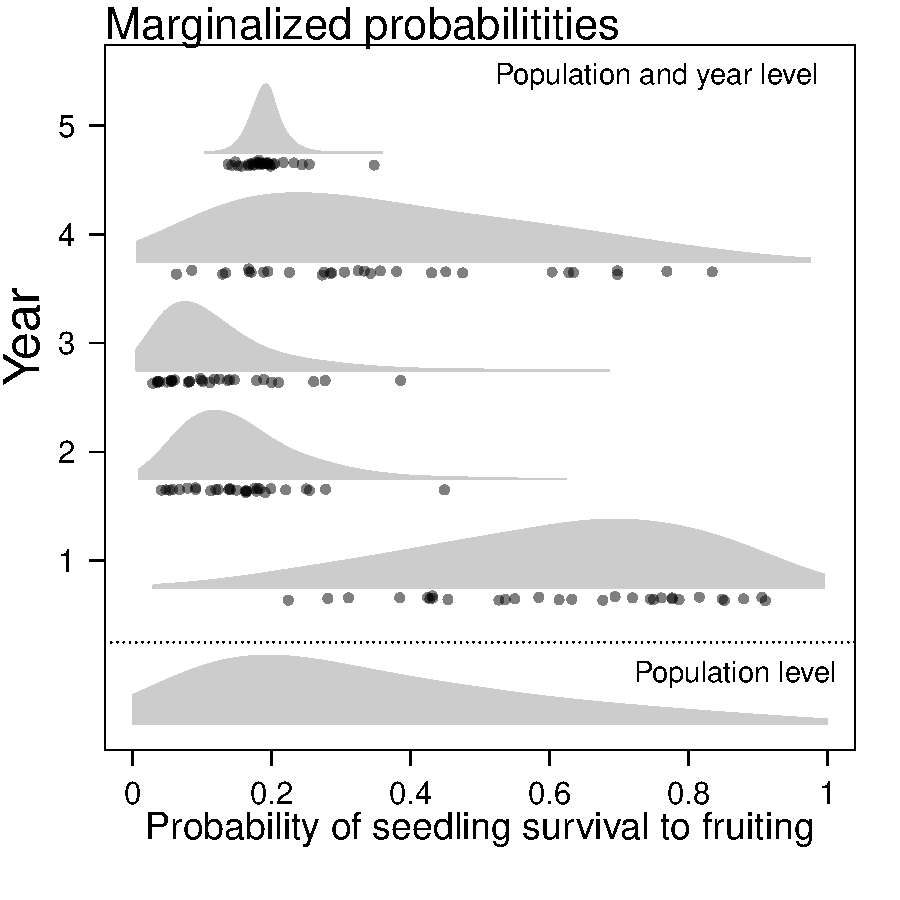
\includegraphics[trim={0 0 0 0},clip,scale=.4]{marginal-posterior}};


\draw [draw, thick] 
  (-3,.5) -- (-3,-2.5) node[midway,yshift=0em,xshift=-7em]{Observations};
\draw [draw, thick]
  (-3,-3) -- (-3,-9) node[midway,yshift=0em,xshift=-7em]{Models};  
  \node [below = .5 cm of d1 ] (a1)  {};
    \node [left = 3.5 cm of d1 ] (a2)  {};
%\draw [draw, thick]
%  (-3,-9.5) -- (-3,-12) node[midway,yshift=0em,xshift=-7em]{Life history};  


\node[rectangle, rounded corners,color=white] (persistence) at (21,-.15)
    {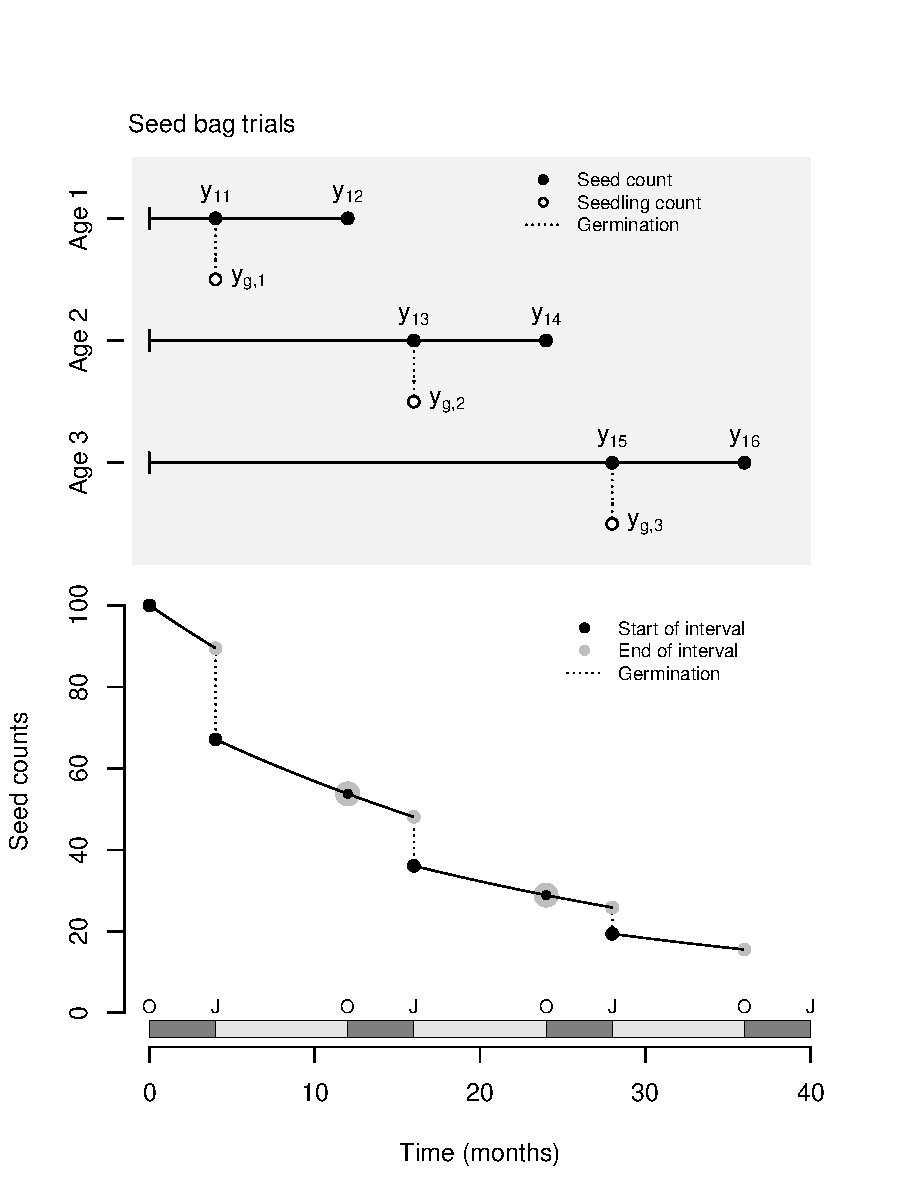
\includegraphics[trim={0cm 11cm 1cm 1.75cm},clip,scale=.65]{../../miscellaneous/conceptual/persistence.pdf}};
\node[] (curve) at (21,-6.5)
    {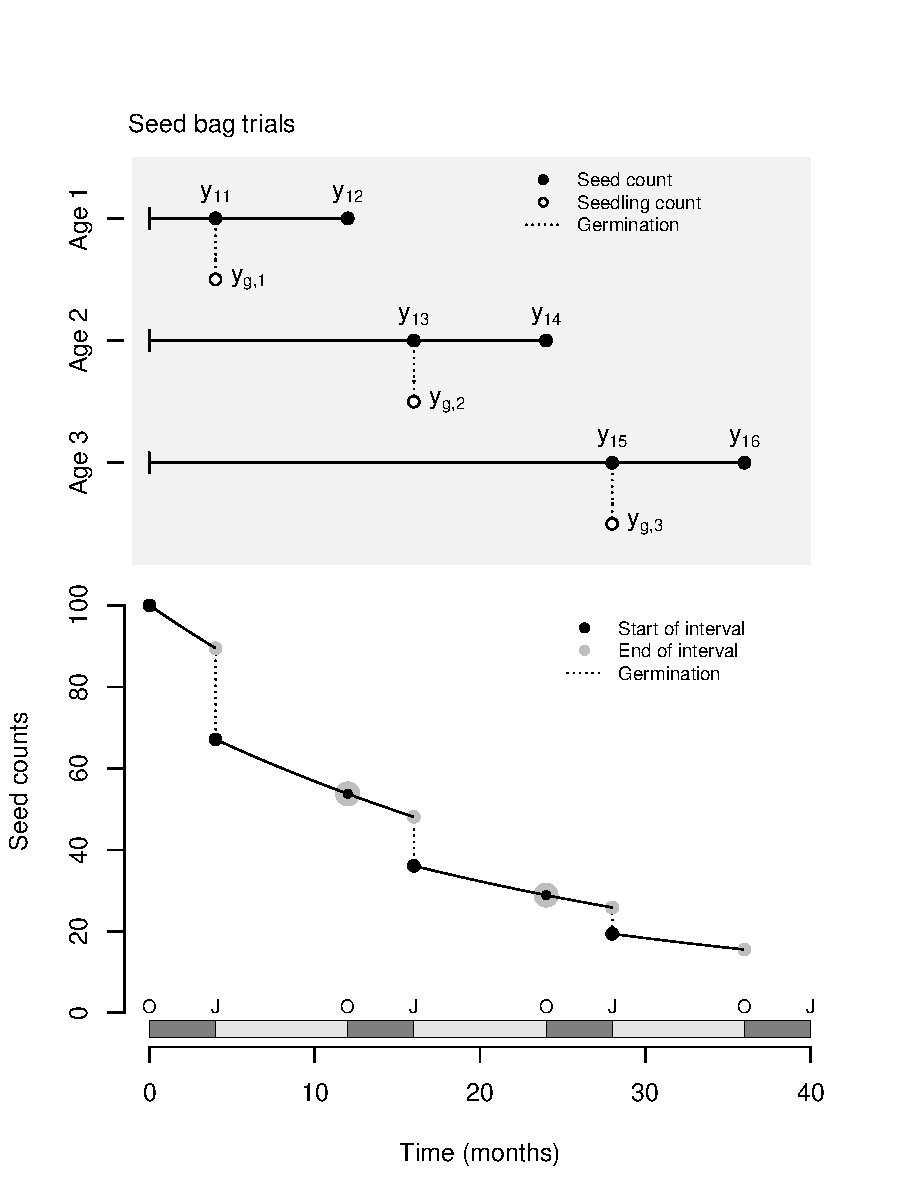
\includegraphics[trim={0cm .5cm 1cm 9.75cm},clip,scale=.65]{../../miscellaneous/conceptual/persistence.pdf}};
\node[] (viability) at (30,-3.5)
    {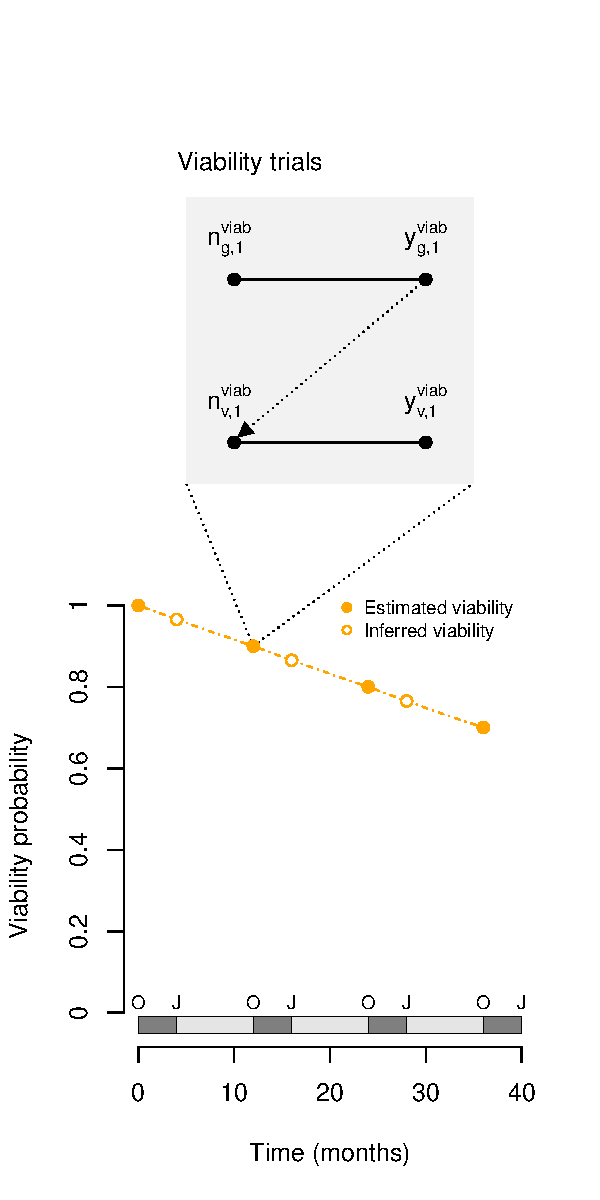
\includegraphics[trim={0 0 1cm 2cm},clip,scale=.65]{  ../../miscellaneous/conceptual/viability.pdf}};    
    
    \draw (15,-9.75)    coordinate (TL) (-2,-9.75) coordinate (O) ;
\draw[brace , very thick] (O)   -- node[box=white,below=3ex]{Annual estimates of seedling survival to fruiting, fruits per plant, seeds per fruit for each study population} (TL);
  

   \begin{scope}[on background layer]
%   \node [fit=(t1) (n3), fill= gray!20, rounded corners, inner sep=.1cm] {};
   \node [fit=(n1) (n4) (d1), fill= gray!30, rounded corners, inner sep=.2cm] {};
   \node [fit=(a1) (A) (H) (sigma) (sigma2), fill= gray!30, rounded corners, inner sep=.2cm] {};
   \node [fit=(sigma), fill= white!30, rounded corners, inner sep=0cm] {};
   \node [fit=(sigma2), fill= white!30, rounded corners, inner sep=0cm] {};
   \node [fit=(persistence), fill= gray!30, rounded corners, inner sep=.1cm] {};
   \node [fit=(curve), fill= gray!30, rounded corners, inner sep=.1cm] {};
   \node [fit=(d3) (a1) (sigma2), draw, very thick, rounded corners, inner sep=.5cm] {};
   \node [fit=(persistence) (viability) (curve), draw, very thick, rounded corners, inner sep=.5cm] {};
   \end{scope}

                
    \end{tikzpicture}
\end{document}